% TODO
% To solve:
% - 4
% To type:
% Done:
% - 1
% - 2
% - 3
% - 5
% Misc:
% - maybe check 5 for thoroughness and format

\documentclass[12pt]{article}

\usepackage{amsmath}
\usepackage{amssymb}
\usepackage{centernot}
\usepackage[margin=2.5cm]{geometry}
\usepackage{tikz}
\usetikzlibrary{arrows, automata, fit}
\tikzset{shorten >=1pt,node distance=2cm,auto,initial text=,accepting/.style={accepting by double, thick}, bend angle=45}
\usepackage{listings}
\usepackage{color}
\usepackage{courier}

\usepackage{fancyhdr}
\pagestyle{fancy}
\lhead{Chang, Gurditta}
\rhead{CSC236 Problem Set 2}

\newcommand{\BigO}{\mathcal{O}}
\newcommand{\N}{\mathbb{N}}
\newcommand{\Z}{\mathbb{Z}}
\newcommand{\Q}{\mathbb{Q}}
\newcommand{\R}{\mathbb{R}}
\newcommand{\I}{\mathcal{I}}
\newcommand{\Lang}{\mathcal{L}}
\newcommand{\Kast}{^\circledast}
\newcommand{\divides}{\mid}
\newcommand{\ndivides}{\centernot \mid}
\newcommand{\cleft}{\mathopen{}\mathclose\bgroup\left}
\newcommand{\cright}{\aftergroup\egroup\right}
\newcommand{\floor}[1]{\left\lfloor #1 \right\rfloor}
\newcommand{\ceil}[1]{\left\lceil #1 \right\rceil}
\newcommand{\ds}{\displaystyle}


\title{CSC236 - Assignment 2}

\author{Ryan Chang, Rikin Gurditta} 
\date{November 11, 2019}

\begin{document}
\maketitle

% \newpage
\section*{Problem 1}
\subsection*{(a)}

This statement is generally true.

\begin{align*}
    \Lang(R^* + S^*) &= \Lang(R^*) \cup \Lang(S^*) \\
    &= \Lang(R)\Kast \cup \Lang(S)\Kast
\end{align*}

Using the provided lemma and the fact that $\Lang(R) \subseteq \Lang(S)$, we know that $\Lang(R)\Kast \subseteq \Lang(S)\Kast$, so $\Lang(R)\Kast \cup \Lang(S)\Kast = \Lang(S)\Kast$.
\begin{align*}
    \Lang((R + S)^*) &= \Lang(R + S)\Kast \\
    &= (\Lang(R) \cup \Lang(S))\Kast \\
    &= \Lang(S)\Kast
\end{align*}

Thus, $\Lang(R^* + S^*) = \Lang((R + S)^*)$, so $R^* + S^* \equiv (R + S)^*$.


\subsection*{(b)}
This statement is not generally true.

\hfill

Suppose $R = S = 0$, then $\Lang(R) = \Lang(S) = \{ 0 \}$, clearly $\Lang(R) \subseteq \Lang(S)$.

Clearly $\Lang(R^* S^*) = \{ 0 \}\Kast$, so $0 \in \Lang(R^* S^*)$. $\Lang((RS)^*) = \{ 00 \}\Kast$, so $0 \notin \Lang((RS)^*)$, so $\Lang(R^* S^*) \neq \Lang((RS)^*)$, so $R^* S^* \not \equiv (RS)^*$.


\newpage
\section*{Problem 2}
\begin{minipage}[c]{0.5\textwidth}
\begin{center}
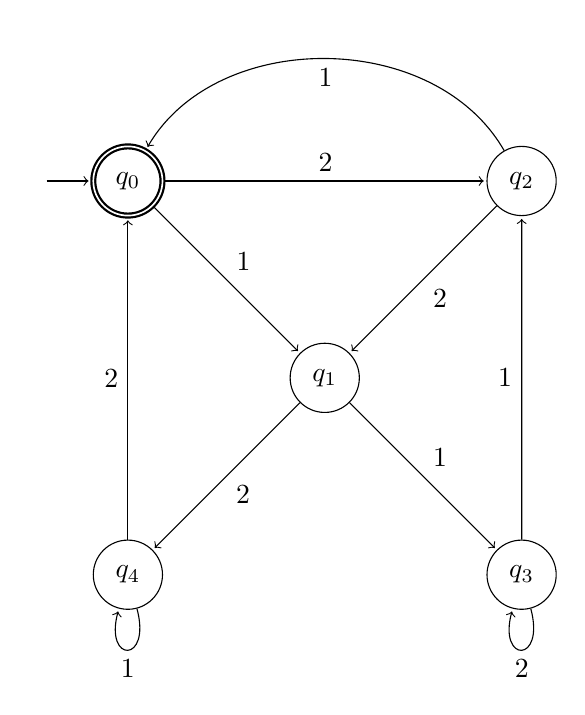
\begin{tikzpicture}[scale=1.25]
    \node[state, initial, accepting] at (0, 0) (0) {$q_0$};
    \node[state] (1) at (2, -2) {$q_1$};
    \node[state] (2) at (4, 0) {$q_2$};
    \node[state] (3) at (4, -4) {$q_3$};
    \node[state] (4) at (0, -4) {$q_4$};
    \path[->]
    	(0) edge node {$1$} (1)
    	(0) edge node {$2$} (2)
    	(1) edge node {$1$} (3)
    	(1) edge node {$2$} (4)
    	(2) edge [bend right=60] node {$1$} (0)
    	(2) edge node {$2$} (1)
    	(3) edge node {$1$} (2)
    	(3) edge [loop below] node {$2$} (3)
    	(4) edge [loop below] node {$1$} (4)
    	(4) edge node {$2$} (0)
    	;
\end{tikzpicture}
\end{center}
\end{minipage}
\begin{minipage}[c]{0.5\textwidth}
\[
\delta^*(q_0, w) = \begin{cases}
q_0, & \text{iff } (val(w) \bmod 5) = 0 \\
q_1, & \text{iff } (val(w) \bmod 5) = 1 \\
q_2, & \text{iff } (val(w) \bmod 5) = 2 \\
q_3, & \text{iff } (val(w) \bmod 5) = 3 \\
q_4, & \text{iff } (val(w) \bmod 5) = 4
\end{cases}
\]
\end{minipage}


\newpage
\section*{Problem 3}
\subsection*{(a)}
\begin{minipage}[t]{0.5\textwidth}
\subsubsection*{i.}
\begin{center}
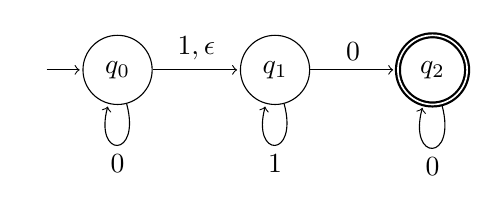
\begin{tikzpicture}
	\node[state, initial]  (0) {$q_0$};
	\node[state] (1) [right of=0] {$q_1$};
	\node[state, accepting] (2) [right of=1] {$q_2$};
	\path[->]
		(0) edge [loop below] node {$0$} (0)
		(0) edge node {$1, \epsilon$} (1)
		(1) edge [loop below] node {$1$} (1)
		(1) edge node {$0$} (2)
		(2) edge [loop below] node {$0$} (2)
		;
\end{tikzpicture}
\end{center}
\end{minipage}
\begin{minipage}[t]{0.5\textwidth}
\subsubsection*{ii.}
\begin{center}
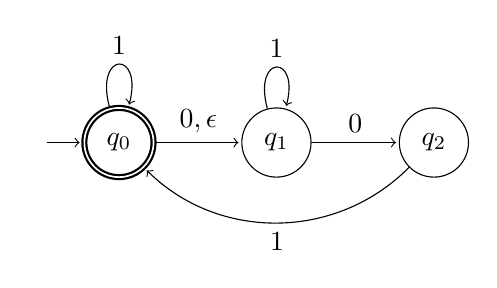
\begin{tikzpicture}
	\node[state, initial, accepting]  (0) {$q_0$};
	\node[state] (1) [right of=0] {$q_1$};
	\node[state] (2) [right of=1] {$q_2$};
	\path[->]
		(0) edge [loop above] node {$1$} (0)
		(0) edge node {$0, \epsilon$} (1)
		(1) edge [loop above] node {$1$} (1)
		(1) edge node {$0$} (2)
		(2) edge [bend left] node {$1$} (0)
		;
\end{tikzpicture}
\end{center}
\end{minipage}

\subsection*{(b)}
\subsubsection*{i.}
\[ (1 (0+1))^* (\epsilon + 1) \]

If the string is cut into pairs of characters starting from the beginning, the first of each pair needs to be a 1, since these are the odd-numbered symbols (if you index the first symbol as the first, instead of the zeroth). The second of the pair can be anything, and there can be any number of these ``pairs", so the expression begins with $(1 (0+1))^*$.

If the string's length is even, it can be cut into pairs so nothing ($\epsilon$) follows the pairs. If the string's length is odd, then the last symbol is an odd position, so it must be a 1. Thus, the expression ends with $(\epsilon + 1)$.

\subsubsection*{ii.}
\[ \epsilon + (0+1) + (0+1)(0+1) + (0+1)^* (0(0+1)(0+1) + 1(01+10+11)) \]

If a string has fewer than 3 symbols then it cannot end with 100, so it should be matched. The regular expression thus begins with $\epsilon + (0+1) + (0+1)(0+1)$.

If the string has at least 3 characters, its beginning can be anything, so the next part begins with $(0 + 1)^*$.

The last three symbols can be any sequence of 3 symbols other than $100$. If the third-last symbol is a $0$, it can be followed by any two symbols, so the end of the string could be matched by $0(0+1)(0+1)$. If the third-last symbol is a $1$, the last two symbols can be anything other than $00$, aka $01$, $10$, or $11$, so the end of the string could also be matched by $1 (01 + 10 + 11)$.

\newpage
\section*{Problem 4}
Since $L$ is regular, there exists a DFA for $L$, which we will refer to as $D = \langle Q_1, \Sigma, \delta_1, s_1, F_1 \rangle$.

Let $Q_2 = Q_1 \cup \{ q_s \}$, where $q_s \notin Q_1$, and let $\delta_2: Q_2 \times \Sigma^* \to \mathcal P(Q_2)$ be defined by:
\[
\delta_2 (q, s) = \begin{cases}
F_1, & \text{iff } q = q_s \text{ and } s = \epsilon \\
\{ q_1 \in Q_1 : \delta_1(q_1, s) = q \}, & \text{iff } q \in Q_1
\end{cases}
\]
(not taking into account the dead states).

Let the NFA $D^R = \langle Q_2, \Sigma, \delta_2, q_s, \{s_1\} \rangle$.

\hfill

\hrule

\hfill

\noindent First, a lemma.

Let $P(n)$: ``for any string $w \in \Sigma^*$ of length $n$, if $q_1 \in Q_1$ and $\delta_1^*(q_1, w) = q_2$, then $q_1 \in \delta_2^*(q_2, w^R)$" where $n \in \N$.

We will prove $\forall n \in \N, P(n)$.

\noindent \textbf{Base case:}

Suppose $|w| = 0$, so $w = \epsilon = \epsilon^R$. Then since $D$ is a DFA, $\delta_1$ has no $\epsilon$ transitions, so for any $q_1 \in Q_1$, $\delta_1^*(q_1, w) = q_1$. Since $w = \epsilon$, we also know that $q_1 \in \delta_2(q_1, w)$, so $P(0)$ holds.

\noindent \textbf{Inductive step:}

(IH) Suppose $n > 0$, and for all $0 \leq k < n$, $P(k)$ holds. That is, for any string $u$ of length $k < n$ and any state $q_1$, if $q_1 \in Q_1$ and $\delta_1^*(q_1, u) = q_2$, then $q_1 \in \delta_2^*(q_2, u^R)$.

Let $w \in \Sigma^*$ have length $n$, then we can write $w$ as $ua$ where $|u| = n - 1$ and $|a| = 1$.

Let $q_2 = \delta_1^*(q_1, u)$, then since $|u| < n$, by the IH $q_1 \in \delta_2^*(q_2, u^R)$.

Let $q_3 = \delta_1(q_2, a)$, then by the definition of $\delta_2$, $q_2 \in \delta_2(q_3, a)$. Also, by the definition of the extended transition, $q_3 = \delta_1^*(q_1, ua)$.

Since $q_2 \in \delta_2(q_3, a)$ and $q_1 \in \delta_2^*(q_2, u^R)$, using the first provided fact we know that $q_1 \in \delta_2(q_3, au^R)$, so if $\delta_1^*(q_1, ua) = q_3$, then $q_1 \in \delta_2^*(q_3, au^R)$.

Thus by the definition of $w^R$, if $\delta_1^*(q_1, w) = q_3$, then $q_1 \in \delta_2^*(q_3, w^R)$. Since $w$ was arbitrary this is true for all strings of length $n$, so $P(n)$ holds.

\hfill

\noindent By the principle of induction, $\forall n \in \N, P(n)$.

\hfill

\hrule

\hfill

Let $w$ be a string in $L$, then since $D$ accepts strings in $L$, $q = \delta_1^*(s_1, w) \in F_1$. Then by the lemma above, $s_1 \in \delta_2^*(q, w^R)$. Furthermore, since $q \in F_1$, there is an $\epsilon$ transition from $q_s$ to $q$ in $D^R$, so $s_1 \in \delta_2^*(q_s, w^R)$ (since the $\epsilon$ transition could be done before the rest of $w^R$ is processed). $s_1$ is an accepting state of $D^R$, so $w^R$ is accepted by $D^R$. Since $w$ was arbitrary, we know that the reverse of any string in $L$ is accepted by $D^R$, so $D^R$ accepts $L^R$.

% Let w be
% {\tiny(We haven't proven that $D^R$ accepts $w^R$ if AND ONLY IF $w^R \in L^R$, but ssshhh)}


\newpage
\section*{Problem 5}

Suppose $L = \{0^n 1^m 2^{n-m} : n \geq m \geq 0 \}$ is regular, then the Pumping Lemma holds. That is, there exists $p \in \N^+$, where if $w \in L$ and $|w| \geq p$, then $\exists x, y, z$ s.t. $w = xyz$, $|xy| \leq p$, $|y| \geq 1$, and $xy^iz \in L$ for all $i \in \N$.

If $w = 0^p 1^p 2^0 = 0^p 1^p$, then clearly $w \in L$ and $|w| \geq p$, so we should be able to "pump" $w$.

Let $x, y, z$ be any strings where $w = xyz$, $|xy| \leq p$ and $|y| \geq 1$. Since the first $p$ symbols in $w$ are $0$s, $x$ and $y$ are entirely made up of $0$s. If $|y| = k$, then $xz = 0^{p-k} 1^p$ (since only $0$s were removed). By assumption of regularity, $xy^0z = xz$ should be in $L$, however $k \geq 1 > 0$ so $p - k < p$, so $xz$ is not in $L$ because there are more $1$s than $0$s. Thus we have reached a contradiction, so $L$ is not regular.

\hfill $\square$


\end{document}